\documentclass[UTF8]{ctexart}  
\usepackage{graphicx}
\title{HW2}
\author{王嵘晟 \quad PB1711614}
\date{}
\begin{document}
	\maketitle
	\section*{3.1-4}
	\par{$2^{n+1}=O(2^{n})$成立,令常数c=2,对任意n$\textgreater$0,有$0\leq2^{n+1}\leq2*2^{n}$}  
	\par{$2^{2n}=O(2^{n})$不成立,假设存在常数c,存在$n_{0}$,对任意n$\ge$$n_{0}$,有$0\leq2^{2n}\leq$$c*2^{n}$则2n$\le$$lgc+n$,即n$\le$lgc,显然与c为常数矛盾。}
	\section*{3.2-3}
	\par{由Stirling公式:n!=$\sqrt{2\pi n}$($\frac{n}{e})^{n}$$(1+\Theta(\frac{1}{n}))$所以lg(n!)=$\frac{1}{2}lg(2\pi n)+n(lgn-lge)+lg(1+\Theta(\frac{1}{n}))$则$\frac{lg(n!)}{nlgn}=\frac{\frac{1}{2}lg(2\pi n)+n(lgn-lge)+lg(1+\Theta(\frac{1}{n}))}{nlgn}=1+\frac{\frac{1}{2}lg(2\pi n)-nlge+lg(1+\Theta(\frac{1}{n}))}{nlgn}$由此可得存在常数$c_{1}$和$c_{2}$和$n_{0}$,使得对任意的n$\ge$$n_{0}$,有$c_{1}nlgn\le lg(n!)\le c_{2}nlgn$,因此式3.19成立。}
	\par{$n!=n*(n-1)*(n-2)*...*1\textless n^{n}=n*n*n*...*n$,所以$n!=o(n^{n})$}
	\par{存在$n_{1}=4$,当$n\ge n_{1}$时,$n!\textgreater 2^{n}$。所以对任意常量$c\textgreater0$,存在常量$n_{0}$,使得对所有$n\ge n_{0}$,有$0\le c*2^{n}\textless n!$,所以$n!=\omega(2^{n})$}
	\section*{4.3-2}
	\par{猜测递归式的解为T(n)=O(lgn),则恰当选择常数c$\textgreater$0,可有T(n)$\le$clgn。首先假定此上界对所有正数m$\le$n都成立,特别是对于m=$\lceil$$\frac{n}{2}$$\rceil$,有T($\lceil$$\frac{n}{2}$$\rceil$)$\le$clg($\lceil$$\frac{n}{2}$$\rceil$)。将其带入递归式,得到}
	\par\noindent{T(n)$\le$clg($\lceil$$\frac{n}{2}$$\rceil$)+1$\le$clg$(\frac{n}{2})+2$}
	\par{=clgn-c+2$\le$clgn}
	\par\noindent{其中只要c$\ge$2,最后一步都会成立。因此T(n)=T($\lceil$$\frac{n}{2}$$\rceil$)+1的解为O(lgn)}
	\section*{4.4-8}
	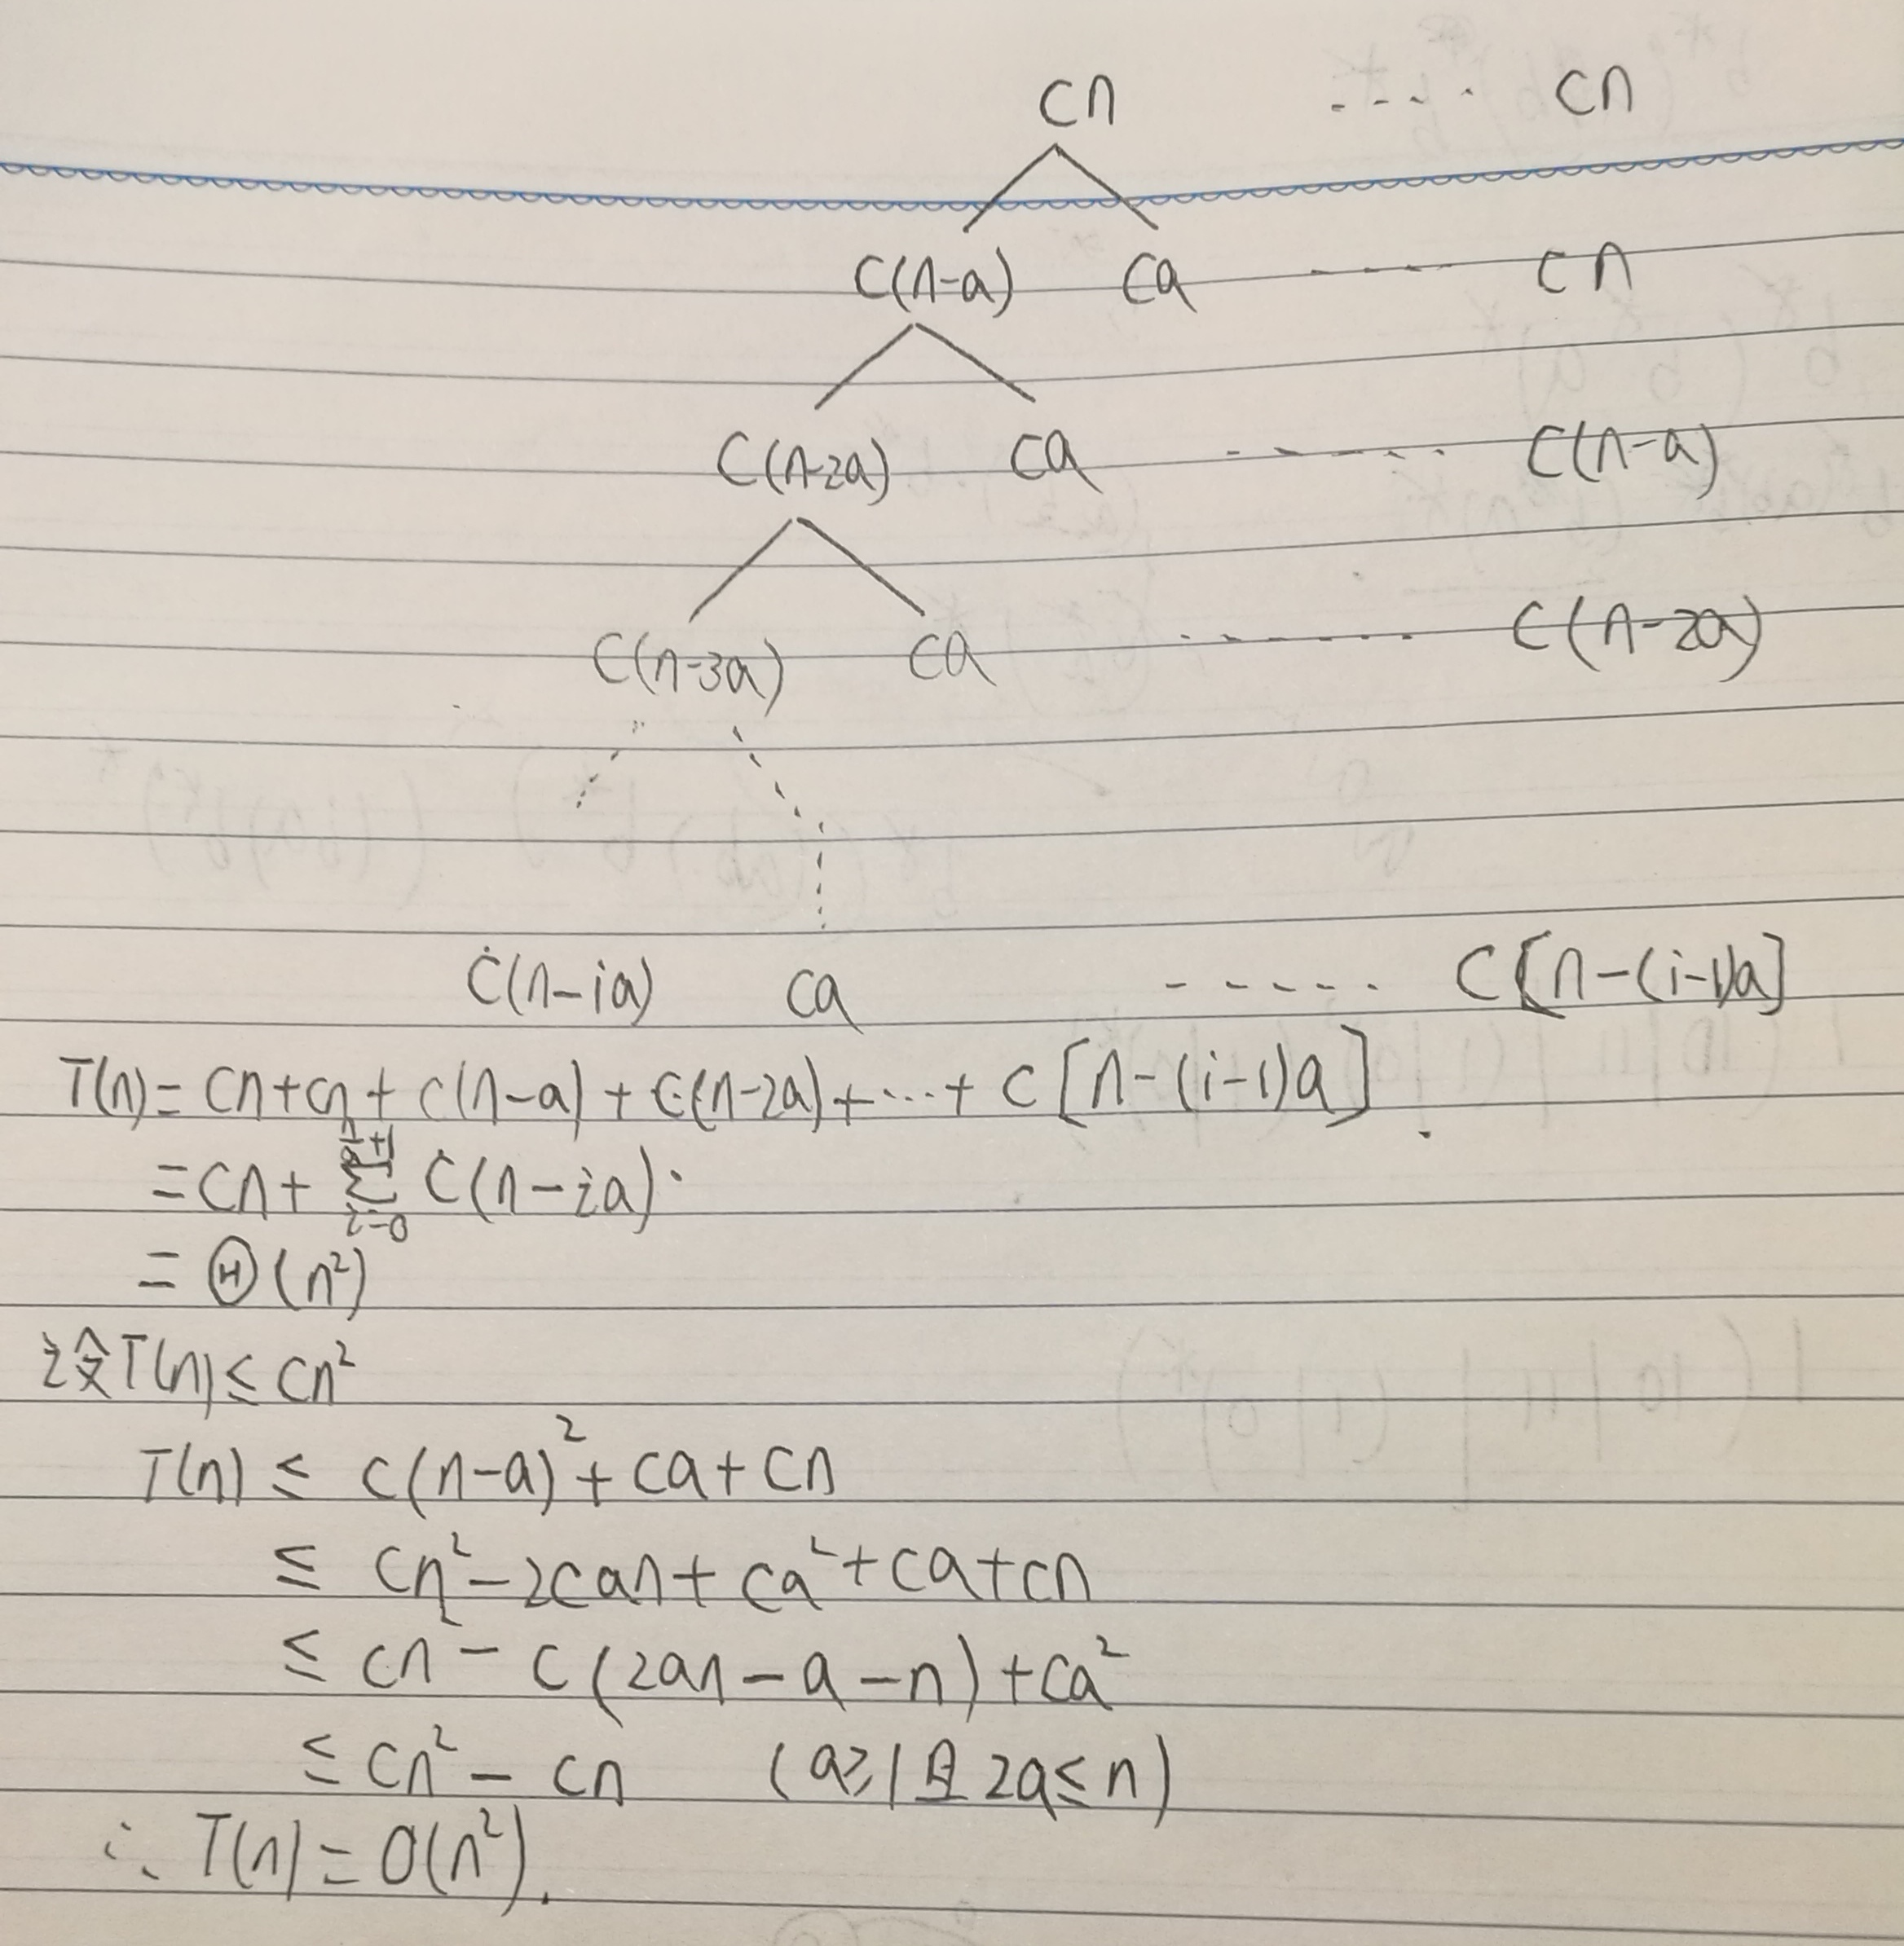
\includegraphics[scale=0.15]{HW2-pic.jpg}
	\section*{4.5-1}
	\noindent{b. T(n)=2T($\frac{n}{4})+\sqrt{n}$}
	\par{f(n)=$\sqrt{n}$,a=2,b=4,显然f(n)=$\Theta$($n^{log_{4}2})=\Theta(n^{\frac{1}{2}})=\Theta(n^{log_{b}a})$,所以由主方法得T(n)=$\Theta(n^{\frac{1}{2}}lgn)$}
	\par\noindent{d.T(n)=2T($\frac{n}{4})+n^{2}$}
	\par{f(n)=$n^{2}$,a=2,b=4。显然f(n)=$\Omega(n^{log_{4}(2+6)})$=$\Omega(n^{2})$即$\varepsilon=6\textgreater0$,且对某个常数c=$\frac{1}{2}$和所有足够大的n有$2*(\frac{n}{4})^{2}\le \frac{1}{2}n^{2}$,所以T(n)=$\Theta(n^{2})$}
	\section*{4.5-4}
	\par{不能,这个递归式对于主方法的三种情况都不适用。但可用以下方法求解递归式}
	
	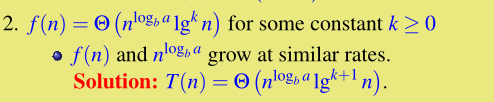
\includegraphics[scale=0.5]{HW2-PIC-2.png}
	\par{a=4,b=2,f(n)=$n^{2}lgn=\Theta(n^{log_{2}4}lgn)$,所以T(n)=$\Theta(n^{2}lg^{2}n)$,所以渐进上界为O($n^{2}lg^{2}n$)}
\end{document}